
\documentclass{article} 
\usepackage{tikz, pgfplots} 
\usetikzlibrary{positioning} 
\usepackage[utf8]{inputenc}
\usepackage{enumerate}
\usepackage{amssymb}
\usepackage{amsmath}  

\begin{document}

\section{Operazioni tra insiemi}
Consideriamo due insiemi \( A \) e \( B \). Le principali operazioni tra
insiemi sono:
\begin{itemize}
	\item \textbf{Unione}: L'unione di due insiemi \( A \) e \( B \), denotata da \( A \cup B \),
	      è l'insieme di tutti gli elementi che appartengono a \( A \) o a \( B \) (o a entrambi). Formalmente,
	      \[
		      A \cup B = \{ x \mid x \in A \text{ o } x \in B \}.
	      \]

	\item \textbf{Intersezione}: L'intersezione di due insiemi \( A \) e \( B \), denotata da
	      \( A \cap B \), è l'insieme di tutti gli elementi che appartengono sia ad \( A \) che a \( B \). Formalmente,
	      \[
		    
		      A \cap B = \{ x \mid x \in A \text{ e } x \in B \}.
	      \]

	\item \textbf{Differenza}: La differenza tra due insiemi \( A \) e \( B \), denotata da
	      \( A \setminus B \), è l'insieme di tutti gli elementi che appartengono a \( A \) ma non a \( B \). Formalmente,
	      \[
		      A \setminus B = \{ x \mid x \in A \text{ e } x \notin B \}.
	      \]

	\item \textbf{Complemento}: Il complemento di un insieme \( A \) rispetto a un insieme
	      universale \( U \), denotato da \( A\setminus U \) o \( \bar{A} \), è l'insieme di tutti
	      gli elementi che appartengono a \( U \) ma non a \( A \). Formalmente,
	      \[
		      A\setminus U = \{ x \mid x \in U \text{ e } x \notin A \}.
	      \]
\end{itemize}

\subsection{Relazioni}

		Una relazione $R_i$ tra due insiemi $A$ e $B$ è un sottoinsieme del prodotto
cartesiano $A \times B$.\\ Ad esempio, siano $A = \{a_1, a_2\}$ e $B = \{b_1,
	b_2\}$. Allora:

\[
	R_i = \{(a_1, b_1), (a_2, b_2)\}
\]

Una relazione può avere proprietà speciali, come:
\begin{itemize}
	\item Riflessiva: $\forall a \in A, (a, a) \in R$
	\item Simmetrica: Se $(a, b) \in R$ allora $(b, a) \in R$
	\item Transitiva: Se $(a, b) \in R$ e $(b, c) \in R$, allora $(a, c) \in R$
\end{itemize}

\subsection{Funzioni}

Una funzione $f: A \to B$ è una relazione che associa ad ogni elemento di $A$
un unico elemento di $B$.\\ La funzione $f$ è:

\begin{itemize}
	\item \textbf{Suriettiva} se $Im(f) = B$.

	      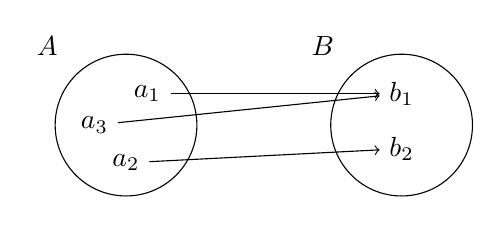
\begin{tikzpicture}
		      \draw(0, 0) circle (0.9cm);
		      \node (a1) at (0.27, 0.4) {$a_1$};
		      \node (a2) at (0, -0.48) {$a_2$};
		      \node (a3) at (-0.4 , 0) {$a_3$};
		      \node (A) at (-1 , 1) {$A$};
		      \draw (3.5,0) circle (0.9cm);
		      \node (b1) at (3.5, 0.4) {$b_1$};
		      \node (b2)at (3.5, -0.3) {$b_2$};
		      \node (B) at (2.5 ,1) {$B$};
		      \draw[->] (a1) -- (b1);
		      \draw[->] (a2) -- (b2);
		      \draw[->] (a3) -- (b1);

	      \end{tikzpicture}
	\item \textbf{Iniettiva} se $\mid f^{-1}(i)\mid =1$, con $i\in B$, $\forall i\in Im(f)$.

	      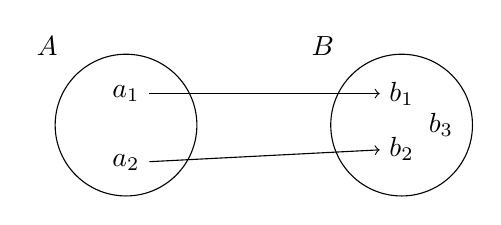
\begin{tikzpicture}
		      \draw (0, 0) circle (0.9cm);
		      \node (a1) at (0, 0.4) {$a_1$};
		      \node (a2) at (0, -0.48) {$a_2$};
		      \node (A) at (-1 , 1) {$A$};
		      \draw (3.5,0) circle (0.9cm);
		      \node (b1) at (3.5, 0.4) {$b_1$};
		      \node (b2)at (3.5, -0.3) {$b_2$};
		      \node (B) at (2.5 ,1) {$B$};
		      \node (b3) at (4 , 0) {$b_3$};
		      \draw[->] (a1) -- (b1);
		      \draw[->] (a2) -- (b2);
	      \end{tikzpicture}
	\item \textbf{Biiettiva} se è sia iniettiva che suriettiva.

	      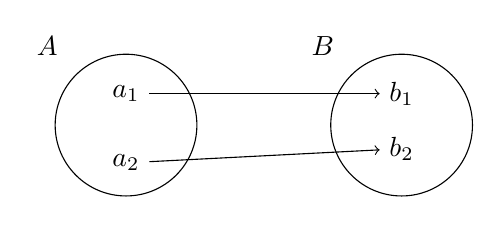
\begin{tikzpicture}
		      \draw (0, 0) circle (0.9cm);
		      \node (a1) at (0, 0.4) {$a_1$};
		      \node (a2) at (0, -0.48) {$a_2$};
		      \node (A) at (-1 , 1) {$A$};
		      \draw (3.5,0) circle (0.9cm);
		      \node (b1) at (3.5, 0.4) {$b_1$};
		      \node (b2)at (3.5, -0.3) {$b_2$};
		      \node (B) at (2.5 ,1) {$B$};
		      \draw[->] (a1) -- (b1);
		      \draw[->] (a2) -- (b2);

	      \end{tikzpicture}
\end{itemize}
\subsection{Relazioni di equivalenza}

Una relazione $R$ su un insieme $A$ è una relazione di equivalenza se soddisfa
le seguenti proprietà:
\begin{itemize}
	\item Riflessiva: $\forall a \in A, (a, a) \in R$
	\item Simmetrica: Se $(a, b) \in R$, allora $(b, a) \in R$
	\item Transitiva: Se $(a, b) \in R$ e $(b, c) \in R$, allora $(a, c) \in R$
\end{itemize}

La classe di equivalenza di un elemento $a \in A$ è definita come:

\[
	[a]_R = \{ b \in A \mid a \sim_R b\}
\]
\newpage
\subsection{Teorema (Unione disgiunta delle classi di equivalenza)}
Ogni insieme è l'unione disgiunta delle sue classi di
equivalenza:$[a]\cup[e]\cup[f]=A$.\\

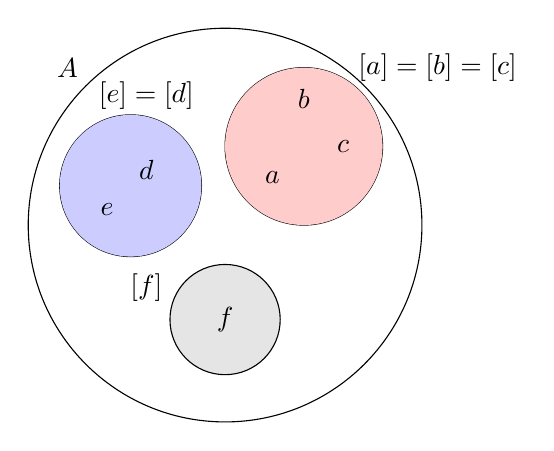
\begin{tikzpicture}
	\draw (4, 0) circle (2.5cm);
	\node (A) at (2, 2) {$A$};
	\fill[gray!20]  (4 , -1.2) circle (0.7);
	\draw (4 , -1.2) circle (0.7);
	\node ([f]) at (3 , -0.8) {$[f]$};
	\draw (2.8 , 0.5) circle (0.9);
	\fill[blue!20] (2.8 , 0.5) circle (0.9);
	\node ([e]) at (3 , 1.65) {$[e]=[d]$};
	\draw (5 , 1) circle (1);
	\fill[red!20] (5 , 1) circle (1);
	\node ([a]) at (6.7 , 2) {$[a]=[b]=[c]$};
	\node (a) at (4.6, 0.6) {$a$};
	\node (b) at (5, 1.6) {$b$};
	\node (c) at (5.5 , 1) {$c$};
	\node (d) at (3, 0.7) {$d$};
	\node (e) at (2.5, 0.2) {$e$};
	\node (f) at (4 ,-1.2) {$f$};
\end{tikzpicture}

\subsection{Insieme Quoziente}

Dato un insieme \( A \) e una relazione di equivalenza \( R \), l'insieme
quoziente è definito come:

\[
	A / R = \{ [a] \mid a \in A \}
\]

dove \( [a] \) è la classe di equivalenza di un elemento \( a \), definita
come:

\[
	[a] = \{ b \in A \mid a \sim_R b \}
\]

Questo significa che gli elementi \( a \) e \( b \) sono equivalenti secondo la
relazione \( R \). L'insieme quoziente \( A / R \) è quindi l'insieme di tutte
le classi di equivalenza generate dalla relazione \( R \).

Consideriamo un insieme \( A = \{1, 2, 3, 4, 5, 6\} \) e una relazione di
equivalenza \( R \) che raggruppa gli elementi in base al resto della divisione
per 2 (numeri pari e dispari). Le classi di equivalenza saranno:

\( [1] = \{1, 3, 5\} \) (numeri dispari)\\
\indent \( [2] = \{2, 4, 6\} \) (numeri pari)

L'insieme quoziente sarà:

\[
	A / R = \{ [1], [2] \}
\]

\newpage
\subsection{Operazioni}
Un \textbf{operazione} n-aria(\(\textasteriskcentered\)) é una funzione del
tipo:
\[
	A_1 \times ... \times A_n \to A_{n+1}\\
\]
\[
	(a_1, ... , a_n) \to \textasteriskcentered(a_1, ...  , a_n)
\]
in particolare se: \\
\[
	A_1 \times ... \times   A_n = A_{n+1} \to \textbf{operazione interna}\\
\]
\[
	n=2 \to \textbf{operazione binaria}
\]
esempio:\\
\[
	\textbf{+}: \mathbb{N} \times \mathbb{N} \to \mathbb{N}\\
\]
\[
	(n_1, n_2) \to n_1 + n_2
\]
\subsection{Struttura algebrica}
La \textbf{struttura algebrica} é una struttura composta da $m$ insiemi ($A_1,
	..., A_m$) e da $n$ operazioni ($\textasteriskcentered_1, ...,
	\textasteriskcentered_n$).
\[
	(A_1, ..., A_m , \textasteriskcentered_1, ..., \textasteriskcentered_n)
\]
\subsection{Gruppo}
Dati $a, b, c \in \mathbb{G}$ e \textasteriskcentered(funzione interna a G):
$\mathbb{G} \times \mathbb{G} \to \mathbb{G}$, un gruppo é una struttura
algebrica del tipo $(\mathbb{G} , \textasteriskcentered)$ che soddisfi tre
proprietá per ogni $a, b ,c \in \mathbb{G}$:
\begin{enumerate}[i.]
	\item Esistenza elemento \textbf{neutro} \underline{$e$} tale che: $e \
		      \textasteriskcentered \ a = a \ \textasteriskcentered \ e = a$.
	\item Esistenza \textbf{inverso} \underline{$a^{-1}$} tale che: $a^{-1}
		      \textasteriskcentered \ a = e$.
	\item \textbf{Associativitá}: $a \ \textasteriskcentered \ (b \ \textasteriskcentered \ c) =
		      (a \ \textasteriskcentered \ b) \ \textasteriskcentered \ c$.
	\item se vale anche la proprietá \textbf{commutativa}: $a \ \textasteriskcentered \ b
		      = b \ \textasteriskcentered \ a$, allora il gruppo si dice: \textbf{Gruppo
		      Abeliano}.
\end{enumerate}
\subsection{Campo}
Sia $\mathbb{K}$ un insieme in cui siano definite le funizoni interne
\textasteriskcentered(+), $\circ(\cdot)$ allora la struttura $(\mathbb{K},
	\textasteriskcentered, \circ)$ é un \textbf{campo} se:
\begin{enumerate}[i.]
	\item $(\mathbb{K}, \textasteriskcentered)$ é un gruppo abeliano con elemento neutro $e$.
	\item definito $\mathbb{K}^{\textasteriskcentered} = \mathbb{K} \setminus \{e\}, \
		      allora \ (\mathbb{K}^{\textasteriskcentered}, \circ)$ é un gruppo abeliano.
	\item vale la proprietà \textbf{distributiva}: $a \circ (b \ \textasteriskcentered \
		      c) = (a \circ b)\ \textasteriskcentered \ (a \circ c) \ $per ogni $a, b, c \in
		      \mathbb{K}$
\end{enumerate}
\subsection{Omomorfismi e isomorfismi}
Date due strutture algebriche, si dice \textbf{omomorfismo} una funzione ($f$)
che commuta con le operazioni, in particolare si ha:
\begin{enumerate}[i.]
	\item \textbf{Omomorfismo di gruppi}:
	      \[
		      (A, \textasteriskcentered_{A}),\ (B, \textasteriskcentered _{B}), \ f: A \to B,
	      \]
	      \[
		      f(a_1 \ \textasteriskcentered_A \ a_2) = f(a_1) \ \textasteriskcentered_A \ f(a_2)
	      \]
	\item \textbf{Omomorfismo di campi}
	      \[
		      (A, \textasteriskcentered_{A}, \circ_A),\ (B, \textasteriskcentered _{B}, \circ_B),  \ f: A \to B:
	      \]
	      \[
		      f(a_1 \ \textasteriskcentered_A \ a_2) = f(a_1) \ \textasteriskcentered_B \ f(a_2)
	      \]
	      \[
		      f(a_1 \circ_A a_2) = f(a_1) \circ_B f(a_2)
	      \]
	\item Una funzione é un \textbf{isomorfismo} se é invertibile, e se la sua funzione
	      inversa ($f^{ -1}$) é a sua volta un omomorfismo.
\end{enumerate}
\section{Matrici}
Dati i due insiemi $M=\{1, 2,..,m\}$ e $N=\{1, 2,..,n\}$ e il campo
$\mathbb{K}$ si definisce \textbf{matrice} una funzione del tipo:
\[
	A: M \times N \to \mathbb{K}
\]
\[
	(i , j) \to a_{ij}
\]
e si indica con:
\[
	A=
	\begin{pmatrix}
		a_{11} & a_{12} & \dots  & a_{1n} \\
		a_{21} & a_{22} & \dots  & a_{2n} \\
		\vdots & \vdots & \ddots & \vdots \\
		a_{m1} & a_{m2} & \dots  & a_{mn}
	\end{pmatrix}
	\in Mat(m,n;\mathbb{K})
\]
$M$ é detto \textbf{insieme delle righe}(m)\\
$N$ é detto \textbf{insieme delle colonne}(n)
\subsection{Esempi notevoli}
\begin{enumerate}[i.]
	\item \textbf{Matrice nulla}
	      \[
		      a_{i,j} = 0, \  \forall (i,j) \in M \times N
	      \]
	      \[
		      O_{3,3} =
		      \begin{pmatrix}
			      0 & 0 & 0 \\
			      0 & 0 & 0 \\
			      0 & 0 & 0
		      \end{pmatrix}
	      \]
	\item \textbf{Matrice identitá}
	      \[
		      a_{i,j} =
		      \begin{cases}
			      1 & \text{se } \ i = j    \\
			      0 & \text{se } \ i \neq j
		      \end{cases}
	      \]
	      \[
		      I_{2,3} =
		      \begin{pmatrix}
			      1 & 0 & 0 \\
			      0 & 1 & 0
		      \end{pmatrix}
	      \]
\end{enumerate}
\subsection{Operazioni}
In $Mat(m , n ; \mathbb{K})$ si definiscono le seguenti operazioni:\\
\begin{enumerate}[i.]
	\item \textbf{Somma}
	      \[
		      +: Mat(m,n;\mathbb{K}) \times Mat(m,n;\mathbb{K}) \to Mat(m,n;\mathbb{K})
	      \]
	      \[
		      ([a_{ij}], [b_{ij}]) \to [a_{ij} +b_{ij}]
	      \]
	\item \textbf{Moltiplicazione per uno scalare}
	      \[
		      \cdot : \mathbb{K} \times Mat(m,n;\mathbb{K}) \to Mat(m,n;\mathbb{K})
	      \]
	      \[
		      (t, [a_{ij}]) \to [t \cdot a_{ij}]
	      \]
	\item \textbf{Prodotto riga per colonna}
	      \[
		      \textasteriskcentered : Mat(m, p  ; \mathbb{K}) \times Mat(p, n ; \mathbb{K}) \to Mat(m, n ; \mathbb{K})
	      \]
	      \[
		      ([a_{ij}] , [b_{ij}]) \to [\sum_{k=1}^{p}a_{ik}\cdot b_{kj}]
	      \]
	\item \textbf{Matrice trasposta};
	      \[
		      A \in Mat(m,n;\mathbb{K}) \implies A^T \in Mat(n,m;\mathbb{K})
	      \]
	      \[
		      (A^T_{ij}) = (A_{ji})
	      \]
\end{enumerate}
\subsection{Proprietà fondamentali delle operazioni con le matrici}

Le seguenti sono le proprietà fondamentali legate alle operazioni sulle
matrici:

\begin{itemize}
	\item \textbf{Somma di matrici}: La somma di due matrici \( A \) e \( B \) di dimensioni
	      compatibili è commutativa e associativa:
	      \[
		      A + B = B + A
	      \]
	      \[
		      (A + B) + C = A + (B + C)
	      \]

	\item \textbf{Prodotto tra una matrice e uno scalare}: Sia \( A \) una matrice e \( \lambda \)
	      uno scalare. Il prodotto di \( \lambda \) con \( A \) soddisfa le seguenti proprietà:
	      \[
		      \lambda (A + B) = \lambda A + \lambda B
	      \]
	      \[
		      (\lambda + \mu) A = \lambda A + \mu A
	      \]
	      \[
		      \lambda (\mu A) = (\lambda \mu) A
	      \]
	      dove \( \lambda \) e \( \mu \) sono scalari e \( A \), \( B \) sono matrici di
	      dimensioni compatibili.

	\item \textbf{Prodotto riga-colonna (prodotto di matrici)}:

	      Le seguenti proprietà sono valide per il prodotto di matrici:

	      \textbf{Associatività}:
	      \[
		      A(BC) = (AB)C
	      \]

	      \textbf{Distributivitá}:
	      \[
		      A(B + C) = AB + AC
	      \]
	      \[
		      (A + B)C = AC + BC
	      \]

	      \textbf{Elemento neutro}:
	      \[
		      A \cdot I_m = I_n \cdot A = A
	      \]

	      \textbf{Omogeneitá }: Per uno scalare \( \lambda \), vale:
	      \[
		      \lambda (AB) = (\lambda A)B = A(\lambda B)
	      \]

	\item \textbf{Matrice trasposta}: Sia \( A \) una matrice di dimensioni \( m \times n \).
	      La trasposta di \( A \), indicata con \( A^T \), è una matrice di dimensioni \( n \times m \), tale che:
	      \[
		      (A^T)_{i,j} = A_{j,i}
	      \]
	      Inoltre, valgono le seguenti proprietà:
	      \[
		      (A^T)^T = A
	      \]
	      \[
		      (A + B)^T = A^T + B^T
	      \]
	      \[
		      (AB)^T = B^T A^T
	      \]
\end{itemize}

\subsection{Metodo di eliminazione di Gauss}

Il metodo di eliminazione di Gauss permette di trasformare una matrice in una
forma più semplice, detta \emph{matrice a scala}, attraverso operazioni
elementari sulle righe. Di seguito sono riportate le definizioni di pivot,
matrice a scala e rango, con esempi.

\begin{itemize}
	\item \textbf{Pivot}: Sia la matrice
	      \[
		      A = \begin{pmatrix}
			      1 & 2 & 3 \\
			      0 & 4 & 5 \\
			      0 & 0 & 6
		      \end{pmatrix}.
	      \]
	      Il pivot della prima riga è \( a_{1,1} = 1 \), il pivot della seconda riga è \(
	      a_{2,2} = 4 \), e il pivot della terza riga è \( a_{3,3} = 6 \). Questi
	      elementi sono i primi non nulli in ciascuna riga. I pivot vengono usati per
	      eliminare gli elementi sotto di loro, come già fatto in questo esempio.

	\item \textbf{Matrice a scala}: Una matrice è in \emph{forma a scala} se soddisfa le seguenti condizioni:
	      \begin{enumerate}
		      \item Le righe nulle sono in fondo.
		      \item I pivot sono allineati a destra rispetto alla riga precedente.
		      \item Gli elementi sotto ogni pivot sono nulli.
	      \end{enumerate}
	      Ad esempio, la matrice
	      \[
		      B = \begin{pmatrix}
			      1 & 2 & 3 & 4 \\
			      0 & 5 & 6 & 7 \\
			      0 & 0 & 8 & 9 \\
			      0 & 0 & 0 & 0
		      \end{pmatrix}
	      \]
	      è in forma a scala perché:
	      - Gli elementi sotto i pivot (1, 5, 8) sono tutti nulli.
	      - I pivot di ogni riga sono allineati a destra rispetto alla riga precedente.
	      - La riga nulla è posizionata alla fine.

	\item \textbf{Rango di una matrice}: Il \emph{rango} di una matrice è il numero di pivot
	      o righe linearmente indipendenti. Per la matrice \( A \) nell'esempio precedente,
	      i pivot sono \( 1 \), \( 4 \) e \( 6 \), quindi \( \text{rank}(A) = 3 \). Per la matrice
	      \[
		      C = \begin{pmatrix}
			      1 & 2 & 3 \\
			      0 & 0 & 0 \\
			      0 & 0 & 0
		      \end{pmatrix},
	      \]
	      abbiamo un solo pivot, \( 1 \), e dunque \( \text{rank}(C) = 1 \).
\end{itemize}
\newpage
\subsection{Operazioni elementari sulle righe}

Durante il metodo di eliminazione di Gauss, si possono eseguire tre tipi di
\emph{operazioni elementari} sulle righe di una matrice per trasformarla in
forma a scala. Queste operazioni non alterano le soluzioni del sistema
associato alla matrice. Le operazioni sono:

\begin{itemize}
	\item \textbf{Scambio di due righe}: Si può scambiare la posizione di due righe, indicato come
	      \( R_i \leftrightarrow R_j \). Ad esempio, scambiando la prima riga con la seconda nella matrice
	      \[
		      A = \begin{pmatrix}
			      1 & 2 & 3 \\
			      4 & 5 & 6
		      \end{pmatrix},
	      \]
	      otteniamo:
	      \[
		      \begin{pmatrix}
			      4 & 5 & 6 \\
			      1 & 2 & 3
		      \end{pmatrix}.
	      \]

	\item \textbf{Moltiplicazione di una riga per uno scalare non nullo}: Una riga può essere
	      moltiplicata per uno scalare \( \lambda \neq 0 \), indicato come \( R_i \to \lambda R_i \).
	      Ad esempio, moltiplicando la prima riga di
	      \[
		      A = \begin{pmatrix}
			      1 & 2 & 3 \\
			      4 & 5 & 6
		      \end{pmatrix}
	      \]
	      per 2, otteniamo:
	      \[
		      \begin{pmatrix}
			      2 & 4 & 6 \\
			      4 & 5 & 6
		      \end{pmatrix}.
	      \]

	\item \textbf{Sostituzione di una riga con la somma di quella riga e un multiplo di un'altra riga}:
	      Si può sommare a una riga un multiplo di un'altra riga, indicato come \( R_i \to R_i + \lambda R_j \).
	      Ad esempio, aggiungendo la prima riga moltiplicata per 2 alla seconda riga di
	      \[
		      A = \begin{pmatrix}
			      1 & 2 & 3 \\
			      4 & 5 & 6
		      \end{pmatrix},
	      \]
	      otteniamo:
	      \[
		      \begin{pmatrix}
			      1 & 2 & 3  \\
			      6 & 9 & 12
		      \end{pmatrix}.
	      \]
\end{itemize}

\subsection{Teorema del metodo di eliminazione di Gauss}

\textbf{Teorema (Eliminazione di Gauss)}:
Sia \( A \) una  matrice di dimensioni \( m \times n \) con coefficienti reali o complessi.
Esiste una sequenza finita di operazioni elementari sulle righe che trasforma \( A \) in una matrice \( A' \)
in forma a scala. In particolare:
\begin{itemize}
	\item La matrice \( A' \) ha lo stesso rango di \( A \).
	\item I pivot nella matrice \( A' \) indicano il numero massimo di righe linearmente
	      indipendenti di \( A \).
\end{itemize}

\section{Metodo di risoluzione di Gauss per sistemi lineari}

\subsection{Definizione di sistema lineare}

Un sistema lineare di \( m \) equazioni in \( n \) incognite è un insieme di
equazioni della forma:

\[
	\begin{cases}
		a_{11}x_1 + a_{12}x_2 + \cdots + a_{1n}x_n = b_1 \\
		a_{21}x_1 + a_{22}x_2 + \cdots + a_{2n}x_n = b_2 \\
		\vdots                                           \\
		a_{m1}x_1 + a_{m2}x_2 + \cdots + a_{mn}x_n = b_m
	\end{cases}
\]

Dove:
\begin{itemize}
	\item \( x_1, x_2, \dots, x_n \) sono le incognite del sistema,
	\item \( a_{ij} \) sono i coefficienti del sistema, per \( i=1,\dots,m \) e \( j=1,\dots,n \),
	\item \( b_1, b_2, \dots, b_m \) sono i termini noti.
\end{itemize}

Possiamo esprimere il sistema in forma matriciale come:

\[
	A \mathbf{x} = \mathbf{b}
\]

dove:
\[
	A = \begin{pmatrix}
		a_{11} & a_{12} & \cdots & a_{1n} \\
		a_{21} & a_{22} & \cdots & a_{2n} \\
		\vdots & \vdots & \ddots & \vdots \\
		a_{m1} & a_{m2} & \cdots & a_{mn}
	\end{pmatrix}, \quad
	\mathbf{x} = \begin{pmatrix}
		x_1    \\
		x_2    \\
		\vdots \\
		x_n
	\end{pmatrix}, \quad
	\mathbf{b} = \begin{pmatrix}
		b_1    \\
		b_2    \\
		\vdots \\
		b_m
	\end{pmatrix}
\]

dove \( A \) è la matrice dei coefficienti, \( \mathbf{x} \) è il vettore delle
incognite e \( \mathbf{b} \) è il vettore dei termini noti.

\subsection{Algoritmo di Gauss}

L'algoritmo di Gauss, o eliminazione gaussiana, è un metodo per risolvere un
sistema lineare tramite trasformazioni elementari sulle righe della matrice
aumentata \( [A | \mathbf{b}] \) del sistema. L'obiettivo è ridurre la matrice
a una forma a scala, da cui sia possibile ottenere le soluzioni con il metodo
della sostituzione all'indietro.

I passi dell'algoritmo sono i seguenti:
\begin{enumerate}
	\item Scrivere la matrice aumentata \( [A | \mathbf{b}] \).
	\item Utilizzare le operazioni elementari di riga per ridurre la matrice a forma
	      triangolare superiore o a scala. Le operazioni elementari consentite sono:
	      \begin{itemize}
		      \item Scambio di due righe,
		      \item Moltiplicazione di una riga per una costante diversa da zero,
		      \item Aggiunta di un multiplo di una riga a un'altra riga.
	      \end{itemize}
	\item Una volta ottenuta la matrice ridotta a scala, si applica la sostituzione
	      all'indietro per ottenere le soluzioni del sistema.
\end{enumerate}

\subsection{Rango della matrice e soluzioni del sistema}

Il numero di soluzioni di un sistema lineare dipende dalla relazione tra il
rango della matrice dei coefficienti \( A \) e il rango della matrice aumentata
\( [A | \mathbf{b}] \). In particolare:
\begin{itemize}
	\item \textbf{Soluzione unica}: Se \( \text{r}(A) = \text{r}(A | \mathbf{b}) = n \), dove \( n \) è il numero di incognite, il sistema ha una soluzione unica.

	      \textbf{Esempio}:
	      \[
		      \begin{cases}
			      x + y + z = 6     \\
			      2x + 3y + 5z = 19 \\
			      3x + 2y + 4z = 17
		      \end{cases}
	      \]
	      La matrice aumentata è:
	      \[
		      \left( \begin{array}{ccc|c}
				      1 & 1 & 1 & 6  \\
				      2 & 3 & 5 & 19 \\
				      3 & 2 & 4 & 17
			      \end{array} \right)
	      \]
	      Riducendo a forma a scala:
	      \[
		      \left( \begin{array}{ccc|c}
				      1 & 1 & 1 & 6 \\
				      0 & 1 & 3 & 7 \\
				      0 & 0 & 1 & 1
			      \end{array} \right)
	      \]
	      Qui \( \text{r}(A) = \text{r}(A | \mathbf{b}) = 3 \), quindi il sistema ha una
	      soluzione unica.

	\item \textbf{Infinite soluzioni}: Se \( \text{r}(A) = \text{r}(A | \mathbf{b}) < n \), il sistema ha infinite soluzioni.

	      \textbf{Esempio}:
	      \[
		      \begin{cases}
			      x + y - z = 0 \\
			      2x + 2y - 2z = 0
		      \end{cases}
	      \]
	      La matrice aumentata è:
	      \[
		      \left( \begin{array}{ccc|c}
				      1 & 1 & -1 & 0 \\
				      2 & 2 & -2 & 0
			      \end{array} \right)
	      \]
	      Riducendo a forma a scala:
	      \[
		      \left( \begin{array}{ccc|c}
				      1 & 1 & -1 & 0 \\
				      0 & 0 & 0  & 0
			      \end{array} \right)
	      \]
	      Qui \( \text{r}(A) = \text{r}(A | \mathbf{b}) = 1 < 3 \), quindi il sistema ha
	      infinite soluzioni, che possono essere espresse in forma parametrica.

	\item \textbf{Nessuna soluzione}: Se \( \text{r}(A) < \text{r}(A | \mathbf{b}) \), il sistema è incompatibile e non ha soluzioni.

	      \textbf{Esempio}:
	      \[
		      \begin{cases}
			      x + y + z = 1 \\
			      x + y + z = 2
		      \end{cases}
	      \]
	      La matrice aumentata è:
	      \[
		      \left( \begin{array}{ccc|c}
				      1 & 1 & 1 & 1 \\
				      1 & 1 & 1 & 2
			      \end{array} \right)
	      \]
	      Riducendo a forma a scala:
	      \[
		      \left( \begin{array}{ccc|c}
				      1 & 1 & 1 & 1 \\
				      0 & 0 & 0 & 1
			      \end{array} \right)
	      \]
	      Qui \( \text{r}(A) = 1 \) mentre \( \text{r}(A | \mathbf{b}) = 2 \), quindi il
	      sistema è incompatibile e non ha soluzioni.
\end{itemize}

\subsection{Teorema di Rouché-Capelli}

Il teorema di Rouché-Capelli fornisce una condizione necessaria e sufficiente
per l'esistenza di soluzioni di un sistema lineare. Esso afferma che un sistema
lineare \( A \mathbf{x} = \mathbf{b} \) è compatibile (ha almeno una soluzione)
se e solo se il rango della matrice dei coefficienti \( A \) è uguale al rango
della matrice aumentata \( [A | \mathbf{b}] \), cioè:

\[
	\text{r}(A) = \text{r}(A | \mathbf{b}).
\]

\subsection{Sistemi lineari omogenei}

Un sistema lineare è detto \emph{omogeneo} se tutti i termini noti sono nulli,
cioè \( \mathbf{b} = \mathbf{0} \). In forma matriciale, un sistema omogeneo è
dato da:

\[
	A \mathbf{x} = \mathbf{0}.
\]

Tali sistemi sono sempre compatibili, in quanto la soluzione banale \(
\mathbf{x} = \mathbf{0} \) è sempre una soluzione. Tuttavia, un sistema
omogeneo può avere anche soluzioni non banali (diverse da zero). La natura
delle soluzioni dipende dal rango della matrice dei coefficienti \( A \):
\begin{itemize}
	\item Se \( \text{r}(A) = n \), l'unica soluzione è quella banale.
	\item Se \( \text{r}(A) < n \), il sistema ha infinite soluzioni.
\end{itemize}

\subsection{Nucleo di una matrice}

Il \emph{nucleo} (o \emph{spazio nullo}) di una matrice \( A \), indicato con
\( \ker(A) \), è l'insieme di tutti i vettori \( \mathbf{x} \) tali che \( A
\mathbf{x} = \mathbf{0} \). In altre parole:

\[
	\ker(A) = \{ \mathbf{x} \in \mathbb{R}^n \mid A \mathbf{x} = \mathbf{0} \}.
\]

Nel contesto di un sistema lineare omogeneo, il nucleo della matrice \( A \)
rappresenta l'insieme delle soluzioni del sistema.

\subsection{Struttura delle soluzioni}

Le soluzioni di un sistema lineare possono essere espresse come somma della
soluzione particolare (se esiste) e della combinazione lineare delle soluzioni
del sistema omogeneo associato. In particolare:
\begin{itemize}
	\item Se il sistema ha una soluzione unica, questa è anche l'unica soluzione del
	      sistema omogeneo associato.
	\item Se il sistema ha infinite soluzioni, esse possono essere espresse come \(
	      \mathbf{x} = \mathbf{x}_p + \mathbf{x}_h \), dove \( \mathbf{x}_p \) è una
	      soluzione particolare del sistema e \( \mathbf{x}_h \) è una soluzione del
	      sistema omogeneo associato.
\end{itemize}

\subsection{Soluzione particolare e interpretazione geometrica}

Consideriamo un sistema lineare \( A \mathbf{x} = \mathbf{b} \). Quando
risolviamo questo sistema, le soluzioni possono essere suddivise in due parti:
\[
	\mathbf{x} = \mathbf{x}_p + \mathbf{x}_h
\]
dove:
\begin{itemize}
	\item \( \mathbf{x}_p \) è una \emph{soluzione particolare}, una soluzione specifica del sistema non omogeneo \( A \mathbf{x} = \mathbf{b} \),
	\item \( \mathbf{x}_h \) è la \emph{soluzione generale del sistema omogeneo associato}, cioè la soluzione del sistema \( A \mathbf{x} = \mathbf{0} \).
\end{itemize}

Quando consideriamo un sistema di due equazioni lineari in tre incognite,
ciascuna equazione rappresenta un piano nello spazio tridimensionale. Le
possibili intersezioni tra due piani danno luogo ai seguenti casi:
\begin{enumerate}
	\item \emph{Intersezione in una retta}: Se i due piani non sono paralleli, essi si intersecano lungo una retta. In questo caso, il sistema ha infinite soluzioni.
	\item \emph{Intersezione in un punto}: Se i due piani sono incidenti in un solo punto (non paralleli e non coincidenti), il sistema ha una soluzione unica.
	\item \emph{Nessuna intersezione}: Se i due piani sono paralleli e distinti, il sistema è incompatibile e non ha soluzioni.
\end{enumerate}
sdkfjsldfsdlf
\end{document}

